\documentclass[prb,preprint]{revtex4-1} 

\usepackage{amsmath}
\usepackage{amsfonts}
\usepackage{graphicx}

\begin{document}

\title{Measuring the Rydberg Constant, Spin-Orbital Coupling Ratio of Mercury, and the Temperature of the Filament of an Incandescent Light Bulb}

\author{Ryan S. Morshead}

\affiliation{Department of Physics, California State Polytechnic University}

\date{\today}

\begin{abstract}

Using a USB4000 Ocean Optics spectrometer along with a fiber optic cable to redirect light from discharge tubes, the spectrums for hydrogen, helium, mercury, a red laser, and an incandescent light bulb were measured. The data from various light sources collected through the spectrometer provides first, a calibration from pixel number to wavelength in addition to the resolution of the spectrometer, and second a calculation for the Rydberg Constant, the magnitude of Spin-Orbital energy splitting in mercury mercury, and the temperature of the tungsten filament in the incandescent lightbulb. The result for the Rydberg constant, $13.6013\pm0.0004$ eV, was found to be in disaagreement with the accepted value of$13.60569253\pm 0.0000000030$ eV . The calculated magnitude of the splitting ratio in mercury, $2.620\pm0.003$, though it was determined to disagree with a value of 2, which was made through simplified theoretical calculations, was still close. And finally, the calculated temperature of the filament, found to be $3222\pm1$ K, is at odds with a measurement of $3153\pm1$ K made with a pyrometer.

\end{abstract}


\maketitle


\section{Introduction}
The idea of the quantum was introduced by the German physicist Max Planck in 1900 in response to the problems posed by the spectrum of radiation produce by hot matter, but the development of quantum theory soon became closely tied to the difficulty of explaining, by classical mechanics, the stability of Rutherford?s nuclear atom\cite{ruth}. Bohr led the way in 1913 with his model of the hydrogen atom which explained the spectral lines predicted by Rydberg's equation\cite{bohr1,bohr2}, but it was not until 1925 that the postulation of Plank's quantum theory found consistent expression in the different, but equivalent, quantum mechanical models developed by Werner Heisenberg, Erwin Schr�dinger, and Paul Dirac\cite{shro,heis,dirac}. In Bohr's model the motion of the electron around the proton in hydrogen was analyzed as if it were a classical problem, mathematically the same as that of a planet around the Sun, but it was additionally postulated that, of all the orbits available to the classical particle, only a discrete set was to be allowed, and Bohr devised rules for determining which orbits they were. In Schr�dinger's wave mechanics the problem is also written down in the first place as if it were a classical problem, but, instead of proceeding to a solution of the orbital motion, the equation is transformed by an explicitly laid down procedure from an equation of particle motion to an equation of wave motion \cite{shro}.

This paper sets out to report on the various properties which are predicted by quantum theory in the hopes of verifying them. For Rydberg and Bohr, the spectrum of hydrogen will be measured to calculate the Rydberg constant with greater precision than could be achieved using an optical grating spectrometer. For Plank, his expression to explain black body radiation will be verified by examining the spectrum produced by a heated filament. And Finally the measurement of the spin-orbit interaction predicted by the initial work of Schrodinger with additions by various others will be measured and quantified.

\newpage

\subsection{Calibration and Resolution}

The USB4000 Ocean Optics spectrometer used for all spectrum measurements in this report comes with a predetermined calibration algorithm to convert pixel numbers to wavelengths in nanometers. However changes in the spectrometer's performance over time will not be accounted for. So without documentation on this algorithm, a known calibration must be used in order to determine error analysis and produce predictable calculations. To accomplish this a voltage is applied to a helium discharge tube to produce its spectrum. By analyzing a series of peaks within a 300 to 800 nm range and comparing them to the known wavelengths of helium's spectral lines a non-linear least squares curve fit of the form,
\begin{equation}\label{eq:eq1}
\lambda = a + b_1p+b_2p^2 ,
\end{equation}
can used to model the data, where $p$ is the pixel number, $a$,$b_1$, and $b_2$ are constants, and $\lambda$ is the wavelength output in nm. The accuracy of this calculation and the error in the calculated wavelengths is then determined by comparing the calibrated pixel data to the known wavelengths. The calibration function found here can be used to for all subsequent calculations of wavelength.

The resolution for the spectrometer was then measured by finding the instrumental linewidth which is defined here to be the full width at half maximum $\sigma_{HM}$ for a monochromatic source. A laser with negligible linewidth is used as the source for this measurement. Thus by definition any two spectral lines that fall within the resolution limit of the spectrometer cannot be resolved to produce reliable data.

\subsection{The Rydberg Constant}

To calculate the value for the Rydberg constant, the calibration function, determined by the previously described analysis of helium's spectral lines, is used to convert  peak pixels measured by the Ocean Optics spectrometer, to wavelengths in nm. After collecting this data, the formula created by Johannes Rydberg to describe the relationship between the discrete spectral lines in hydrogen written as
\begin{equation}
E_{\gamma}=\frac{hc}{\lambda}=E_R\left(\frac{1}{n'^2}-\frac{1}{n^2}\right) ,
\label{eq2}
\end{equation}
where $n$ and $n'$ are the principle quantum number for the orbital energies of hydrogen and $E_{\gamma}$ is the energy of the photon produced by the resulting change in orbital potential, can be manipulated to fit the form $y=mx+b$. In this configuration the Rydberg equation yields
\begin{equation}
\lambda=\frac{hc}{E_R}\left(\frac{1}{n'^2}-\frac{1}{n^2}\right)^{-1},
\label{eq:eq3}
\end{equation}
where $\lambda=y$, $(hc)/E_R=m$, and the remaining term is equal to $x$. The calculated wavelengths from the observed spectrum can then be used in tandem with the $n$ values for the corresponding orbital potentials to perform a least squares optimization of the values for $m$ and the $y$-intercept, $b$. In order to perform this operation though the $n'$ term must be limited to a single value in order to produce a linear curve which is dependent on a single variable. By setting $n'$ equal to $2$ our comparison of spectral line measurements is limited to the Balmer series. Thus by confining our measurements to this collection of orbital potential variations, the optimized value for $m$ can be determined. The form of $m$ can then be altered to give

\begin{equation}
E_R=(hc)/m.
\end{equation}

\subsection{Spin-Orbital Energy Splitting}

Determining the spin-orbital energy for mercury requires the same method of measurement used to find the peak wavelengths for hydrogen. Thus the collection of $\lambda$ values gathered from the spectrum of mercury, can be related to their corresponding theoretically calculated values in order to verify the theory that generated them. However because The Bohr Model, and consequently The Rydberg Equation, do not accurately describe the emission spectra of elements with heavier nuclei with higher charger and more electrons, a more rigorous method must be used to model the atomic structure of mercury in order for a useful comparison to be drawn.

To begin developing this model we recognize a number of things -- first that electrons have a magnetic moment $\vec{\mu}$ as a result of their spins $\vec{S}$ where $\vec{\mu} \propto \vec{S}$ with $\vec{S}$ for electrons having a magnitude of either $\pm1$ by Pauli exclusion principles. Second that the nucleus of an atom, from the perspective of an orbiting electrons rest frame, appears to be orbiting the electron. From these two facts we can see that the apparent orbit of the central charge about the electron produces a magnetic field $\vec{B}$ which is proportional to the orbital angular momentum $\vec{L}$ and that this magnetic field has a potential energy E which is proportional to  $\vec{\mu}\cdot\vec{B}$. Thus the magnetic energy which arrises from the interaction between the magnetic moment of electrons and the magnetic field generated by the relative motion of an atom's central charge can be written as
\begin{equation}\label{eq:eq5}
E_{s-o} = A \vec{S} \cdot \vec{L},
\end{equation}
where A is proportionality constant. The value for this spin-orbital energy is not only dependent on the magnitude of $\vec{S}$ and $\vec{L}$ but also on the orientation of the vectors. Then by taking the square of the total angular momentum, $\vec{J} = \vec{L} + \vec{S}$, the resulting expression can then be rearranged to solve for $\vec{S} \cdot \vec{L}$ in the final form where
\begin{equation}\label{eq:eq7}
J^2=\vec{J} \cdot \vec{J} = L^2+S^2+2\vec{S} \cdot \vec{L}\implies\vec{S} \cdot \vec{L} = \frac{1}2(J^2-L^2-S^2).
\end{equation}
Then using the fact that the allowable values for $J^2$, $L^2$, and $S^2$ are of the form
\begin{equation}\label{form}
y^2=\hbar\sqrt{y(y+1)}
\end{equation}
where $y$ is used in place of the values for the quantum numbers $J$,$L$, and $S$ of a particular state, a final expression for the Energy associated with spin-orbital interactions can be written as
\begin{equation}\label{Ej}
E_{s-o} = \frac{A\hbar^2}2 \left(J(J+1)-L(L+1)-S(S+1)\right).
\end{equation}
Ultimately this expression can be used to find a theoretical value for the ratio of the energies associated with different orientations of $\vec{S}$ and $\vec{L}$ by the expression
\begin{equation}\label{ratio}
Q_E=\frac{E_{J=2}-E_{J=1}}{E_{J=1}-E_{J=0}},
\end{equation}
where $E_J=E_{s-o}$ using different, but allowable values of J. Thus with the final measured values for the energy splitting of mercury and the final theoretical values determined through the previously described model the two values can be compared. The result of this comparison will show whether the theoretical model used accurately describes the structure of heavier elements like mercury which contain nuclei with relatively high central charges and many electrons.

\subsection{Filament Temperature}

To measure the temperature of the tungsten filament in an incandescent light bulb two methods are employed; the first being a direct measurement of the temperature using an optical pyrometer which applies an internally calibrated lamp and filter to output overlaid monochromatic light from the calibrated lamp and the target. Adjusting the temperature of the lamp by changing the current running to the calibrated lamp allows the user to match the the unique color of the target through a particular filter to the color of light produced by the lamp through that same filter.

The second method uses the Ocean Optics spectrometer to measure the spectrum produced by the filament. Collecting the relative intensities associated with each wavelength of light then gives data which can be fit to a curve. Because the filament is a crystaline transition metal the electrons in the filament of the lightbulb are dissociated. Then the force they experience as a result of the voltage which is applied causes them to accelerate towards any relative positive charge. However as they travel through the material they collide with the nuclei of the filament transferring some kinetic energy and thus increasing the temperature of the material in the process. This increase in temperature induces thermal radiation which is electromagnetic radiation generated by the thermal motion of charged particles in matter. This radiation then, is not dependent on orbital potentials of atoms, and produces a continuous distribution of wavelengths which are associated with the temperature of the object, where temperature is by definition the average of all individual kinetic energies. As a result, Max Plank's model for the intensity of black body radiation,
\begin{equation}\label{blackbody}
I(E)=\frac{AE^5}{e^{E/(k_BT)}-1},
\end{equation}
where $I$ is the relative intensity, $E$ is the energy of each photon and $T$ is the temperature of the light source in kelvin, and $A$ is a constant, can be used to model the spectrum produced by the filament. A calculated value for $T$ can then be determined by using a least squares optimization of the values for $T$ and $A$ in equation \eqref{blackbody}.



\section{Results and analysis}

\subsection{Calibration and Resolution}

The calculated wavelengths produced through the calibration function described earlier, pixel numbers, and their corresponding known wavelengths are compared in Table \ref{helium} while the least squares optimization function which was used to define that function is shown in Fig \ref{calibration}. The resolution of the spectrometer defined to be $\sigma_{HM}$, was found to be $1.7\pm0.1$ after analyzing the single peak produced by red laser with a measured wavelength of $633.5\pm0.1$.

\newpage

\begin{table}[h!]
\caption{Measured pixel numbers, calibrated wavelengths, and known wavelengths of helium's spectrum.}
\begin{ruledtabular}
\begin{tabular}{c c c c c}
&$p$&$\lambda \pm 0.1$ (nm)&$\lambda$ known (nm)&
\\
\hline
&1004&388.7&388.86&\\
&1294&447.3&447.14&\\
&1415&471.4&471.31&\\
&1520&492.3&492.19&\\
&1567&501.5&501.57&\\
&2009&587.5&587.57&\\
&2433&667.7&667.81&\\
&2642&706.5&706.52&\\
&2761&728.3&728.13&\\
\end{tabular}
\end{ruledtabular}
\label{helium}
\end{table}

\begin{figure}[h!]
\centering
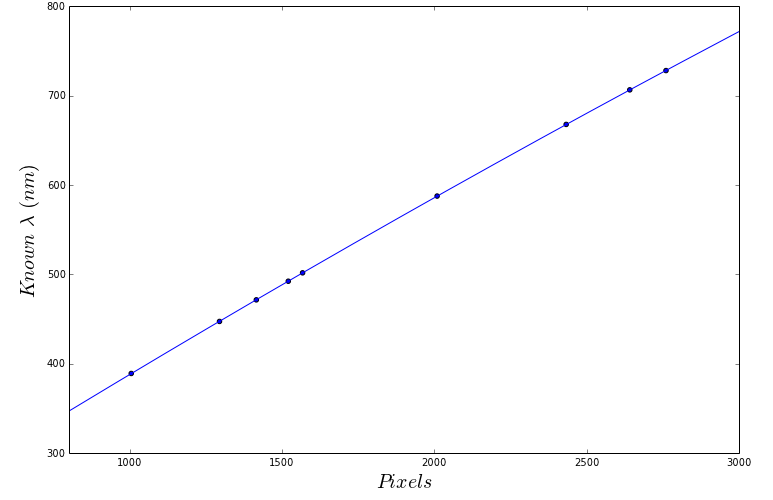
\includegraphics[width=\textwidth]{calibration.png}
\caption{Values of q on each drop with falling and forced fall values}
\label{calibration}
\end{figure}

\newpage

\subsection{The Rydberg Constant}
With peak pixel data collected from the Ocean Optics Spectrometer spectrometer and then converted into wavelengths by means of the calibration function, the least squares optimization of Eq. (3) was used to find the value of $(hc)/ER$ which best fit the data. The final results for the $\lambda$ values and the corresponding energies $E_\gamma$ are shown by Table \ref{table II}. The linear curve fit used to find $E_R$ is shown by Fig. \ref{lincurve}.

The final value, $13.6013\pm0.0004$ eV, for The Rydberg Constant was not in agreement with the accepted value of $13.60569253\pm0.0000000030$ eV even though our values using the spectrometer had an additional significant figure to our accuracy as compared to $\lambda_{pref}$ values which were made with an optical grating spectrometer. Though the y intercept of -0.035 nm for the fit function is not zero it falls within our 0.1 nm margin of error and does not imply any significant source of systematic error.

\newpage

\begin{table}[h!]
\caption{Hydrogen.}
\begin{ruledtabular}
\begin{tabular}{c c c c}
&$\lambda \pm 0.1$ (nm)&$\lambda_{prev}$&
\\
\hline
&410.0&-\\
&434.0&438$\pm7$&\\
&486.1&486$\pm1$&\\
&656.3&657$\pm1$&\\
&777.7&-\\
\end{tabular}
\end{ruledtabular}
\label{table II}
\end{table}

\begin{figure}[h!]
\centering
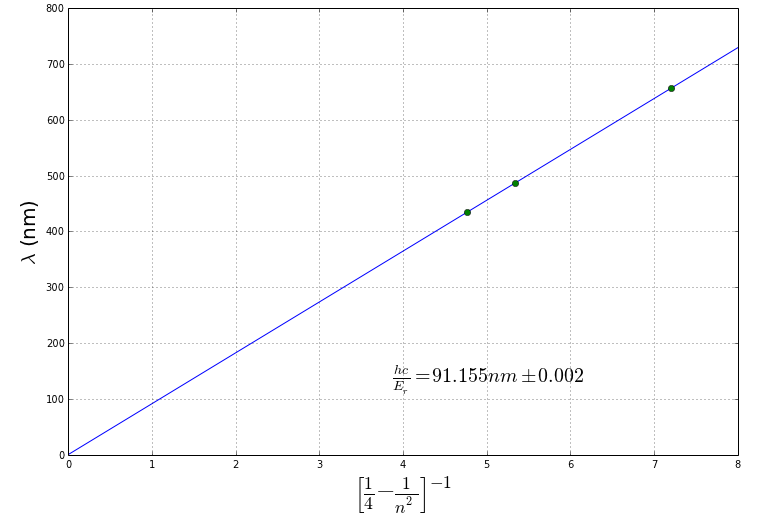
\includegraphics[width=\textwidth]{rydberg.png}
\caption{Values of q on each drop with falling and forced fall values}
\label{lincurve}
\end{figure}

\newpage

\subsection{Spin-Orbital Energy Splitting}

The wavelengths and energies associated with the mercury spectrum can be found in Table\ref{mercury}. From these energies the ones which corresponded to $E_J$ with J values of 0,1,2 were identified and entered into Equation \eqref{ratio} to compute the measured value of the spin-orbit energy splitting ration for mercury.

\begin{table}[h!]
\caption{The wavelengths, energies, and identified transition associated with the peak pixels resulting from the spectrum of mercury}
\begin{ruledtabular}
\begin{tabular}{c c c c c}
&$\lambda \pm 0.1$ (nm)&$E_{\gamma}$ (eV)& Transition
\\
\hline
&435.9&2.8446$\pm.0007$&$6s7s7^3S_1 \rightarrow 6s6p^3P_1$\\
&486.1&2.5505$\pm.0005$&$6s8s8^1S_0 \rightarrow 6s6p6^1P_1$\\
&546.0&2.2710$\pm.0004$&$6s7s7^3S_1 \rightarrow 6s6p6^3P_2$\\
&576.7&2.1499$\pm.0004$&$6s6d6^1D_2 \rightarrow 6s6p6^1P_1$\\
&578.8&2.1420$\pm.0004$&$6s6d6^3D_1 \rightarrow 6s6p6^1P_1$\\
\end{tabular}
\end{ruledtabular}
\label{mercury}
\end{table}

The final value of the ratio, which used transitions of $6s7s7^3S_1 \rightarrow 6s6p^3P_1$ for $E_2$, $6s7s7^3S_1 \rightarrow 6s6p6^3P_2$ for $E_1$, and a known value of $4.6658\pm0.0002$ eV for $E_0$ was found to be $2.620\pm0.003$. This strongly disagreed with the theoretically determined value of 2 which arose from Equation \eqref{Ej}. However, because there is no obvious reason to rule out the measurements which were made, it's likely that the model used to produce the theoretical calculation is not rigorous enough. 

\newpage

\subsection{Filament Temperature}

The direct measurement and the blackbody curve fit used to identify the temperature of the filament result in two independent values that can be compared against each other in order to verify the calculated temperature from the curve fit. The actual graph of the least squares optimization of $T$ and $A$ is show in Fig. \ref{blackbody}.

\begin{figure}[h!]
\centering
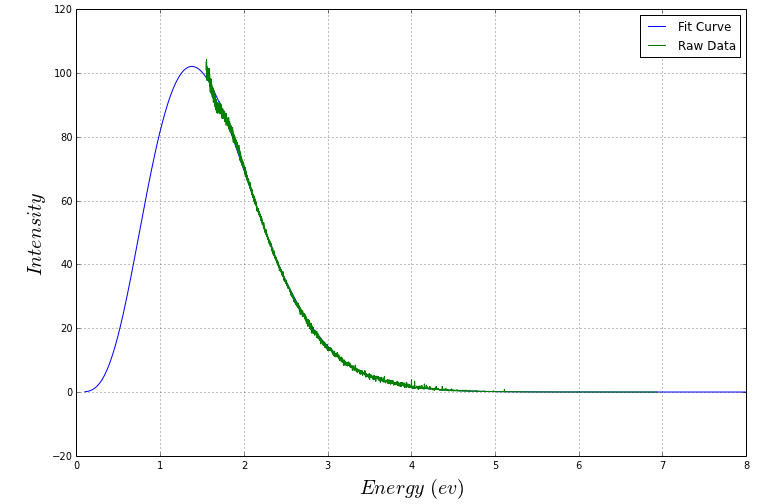
\includegraphics[width=\textwidth]{blackbody.png}
\caption{The spectrum produced by the tungsten filament in a lightbulb and the curve fit based on Plank's black body equation.}
\label{blackbody}
\end{figure}

The temperature determined through the least squares optimization came out to be $3222\pm1$ K while the temperature measured using the pyrometer, and which conflicts with the calculated value, is $3153\pm1$ K. However we can rule out the measurement made by the pyrometer as the calibrated lamp inside the pyrometer was not able to accurately match the color of the observed light from the source; the temperature knob controlling the current to the lamp reached its limit shortly before the colors could be made indistinguishable in the viewer. As a result the temperature measured using the pyrometer is markedly less that the one made using the spectrum and least squares optimization.

\newpage

\section{Conclusion}

This report aimed to measure a variety of variables; the Rydberg constant with greater accuracy than could be achieved previously using an optical grating spectrometer; the spin orbital coupling ratio in order to investigate the rigor of the model used to calculate its theoretical value, and the temperature of an incandescent light bulb filament. The respective values of $13.6013\pm0.0004$ eV, $2.620\pm0.003$, $3222\pm1$ K can be said to have met that aim. Though the Rydberg constant does not agree with accepted value and the spin-orbit splitting ratio for mercury and the temperature of the filament do not agree with their alternate values, what has been reported on the splitting ratio and filament temperature still remains legitimate due to the possibility of an inaccurate theoretical model in the case of mercury, and an over saturated pyrometer in the case of the filament.

\newpage

\begin{acknowledgments}

Coffee, coffee, coffee, coffee, coffee, coffee, coffee, coffee, coffee, coffee, coffee, coffee, coffee, coffee, coffee, coffee, coffee, coffee, coffee, coffee, coffee, coffee, coffee, coffee, and more coffee.

\end{acknowledgments}


\begin{thebibliography}{99}

\bibitem{const}  P.J. Mohr, B.N. Taylor, and D.B. Newell (2011), ``The 2010 CODATA Recommended Values of the Fundamental Physical Constants" (Web Version 6.0).

\bibitem{ruth} Rutherford E. (1911). ``The Scattering of Alpha and Beta Particles by Matter and the Structure of the Atom". Philosophical Magazine, Series 6 \textbf{21}: 669-688.

\bibitem{bohr1} Niels Bohr (1913). ``On the Constitution of Atoms and Molecules, Part I". Philosophical Magazine \textbf{26} (151): 1-24.

\bibitem{bohr2} Niels Bohr (1913). ``On the Constitution of Atoms and Molecules, Part II Systems Containing Only a Single Nucleus". Philosophical Magazine \textbf{26} (153): 476-502.

\bibitem{shro} Schrodinger, Erwin (December 1926). ``An Undulatory Theory of the Mechanics of Atoms and Molecules". \textit{Phys. Rev.} \textbf{28} (6): 1049-1070.

\bibitem{heis} Aitchison, et al., ``Understanding Heisenberg's 'magical' paper of July 1925: a new look at the calculational details," Am. J. Phys. \textbf{72}, 1370 (2004)

\bibitem{dirac} Dirac, P. A. M. (1930). ``A Theory of Electrons and Protons". Proceedings of the Royal Society A: Mathematical, Physical and Engineering Sciences \textbf{126} (801): 360, \textbf{117} (778): 610. 

\end{thebibliography}

\end{document}
